\documentclass{cumcmthesis}
%\documentclass[withoutpreface,bwprint]{cumcmthesis} %去掉封面与编号页
%\usepackage{graphicx}
%\usepackage{subfigure}
\usepackage{tabularx}
\title{论文题目}
\tihao{C}            % 题号
\baominghao{202217241200}    % 报名号
\schoolname{华中科技大学}
\membera{卢凯}
\memberb{陈铭锐}
\memberc{房怿宽}
\supervisor{胡勇}
\yearinput{2022}     % 年
\monthinput{09}      % 月
\dayinput{15}        % 日

\begin{document}
	\maketitle
	\begin{abstract}
		摘要的具体内容。
		\keywords{关键词1\quad  关键词2\quad   关键词3}
	\end{abstract}
	%\tableofcontents
	
	
%----------- 正文 ----------
%----------- 一、问题重述 ----------
	\section{问题重述}
		\subsection{问题背景}
		\par 
		\subsection{待求解的问题}
		\par 
			\begin{enumerate}
				\item{问题一:}
				\item{问题二:}
				\item{问题三:}
			\end{enumerate}
%----------- 二、问题分析 ----------
	\section{问题分析}
		\subsection{问题一:}
		\subsection{问题二:}
		在问题二中,我们首先假设对于任意的$D_i$,通过测量$D_0,D_1,D_j$三个无人机的位置,得到两个小角$\alpha_1,\alpha_2$,进而能够确定自己在$D_0 - D_1$坐标系中的位置。
		
		可以假定的是,对于任意的$D_i$,在接收其他无人机的发射信号时,有以下公共知识:
		\begin{itemize}
			\item	位置待定无人机自身的编号$i$,
			\item	可以辨识从$D_0$与$D_1$发出的信号,但不确定第三个信号来源,
			\item	无人机机群的结构,即各个编号无人机在圆上的大致位置与顺序,任意两个无人机不能交换顺序,
			\item 	待定无人机相对于理想位置的偏差较小,即$ {\lVert \omega_i \rVert}^2 < r_0 $.
		\end{itemize}
		\begin{figure}[htb]
			\centering
			\subfloat[组态1]{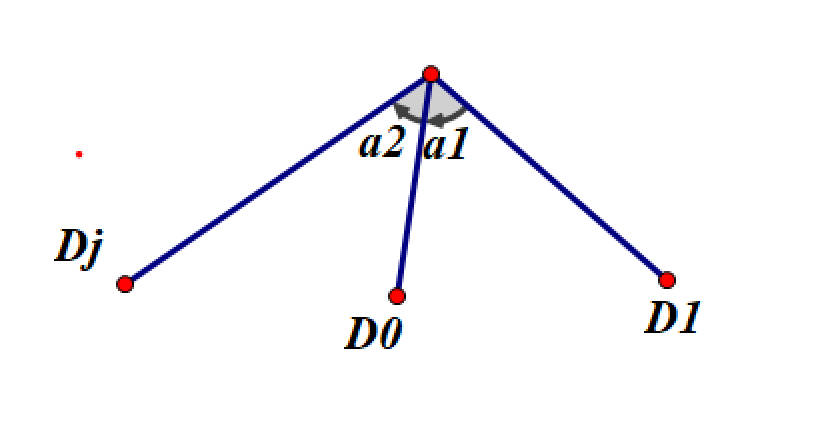
\includegraphics[width=0.4\linewidth]{../figures/1}}
			\subfloat[组态2]{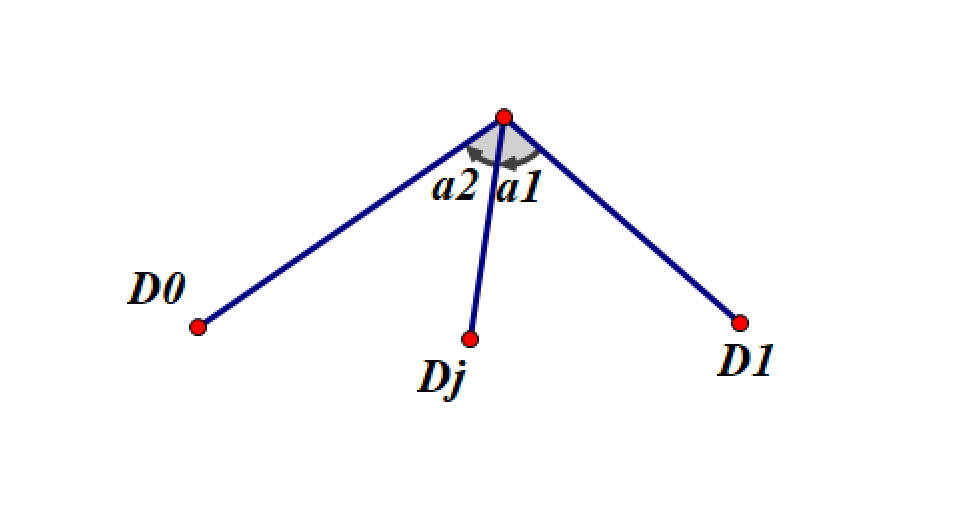
\includegraphics[width=0.4\linewidth]{../figures/2}}
			\caption{可能出现的两种组态}
			\label{fig1}
		\end{figure}
		基于以上公共知识,需要设计算法$D_i = f(\alpha_1, \alpha_2)$求解$D_i$在$D_0 - D_1$坐标系中的位置。
		\subsection{问题三:}
%----------- 三、模型的假设与约定 ----------
	\section{模型的假设与约定}
		\begin{itemize}
			\item{} one
			\item{} two
			\item{} three
		\end{itemize}
%----------- 四、符号说明及名词定义 ----------
	\section{符号说明及名词定义}
		\begin{center}
			\begin{table}[h]
				\caption{本论文所使用的符号}
				\begin{tabularx}{\textwidth}{p{0.08\textwidth}X}
					\toprule	
					
					$D_i$ & 编号为$i$的无人机的理想位置  \\
					$\widehat{D_i}$ & 编号为$i$的无人机的有偏实际位置  \\
					$D_i(\rho,\theta)$ & 用极坐标表示的无人机的位置 \\
					  
					$\overrightarrow{D_iD_k}$ & 从$D_i$指向$D_k$的矢量 \\
					$\omega_i$      & 编号为$i$的无人机的误差矢量,即$\overrightarrow{\widehat{D_i}D_i}$ \\
					$\bigodot O_i$    & 第$i$个理想圆  \\
					
					$hc_k$     & Holding cost of product k per unit and period;holding cost of product k per unit and period;holding cost of product k per unit and period   \\
					$hc_k$     & holding cost of product k per unit and period   \\
					oc   & overtime costs per unit   \\
					$M_{kt}$   & bignumber for product k in period t\\
					$pc_{k}$   & production cost of product k per unit\\
					$pc^r_{k}$ & remanufacturing cost of product k per unit\\
					$sc_{k}$   &  setup cost of product k\\
					$sc^r_{k}$ &  setup cost of returned product k\\
					$tp_{k}$   &  production time for one unit of product k\\
					$tp^r_{k}$ & remanufacturing time for one unit of product k\\
					$ts_{k}$   & setup time of product k\\
					$ts^r_{k}$ & setup time of returned product k\\
					
					 
					$BL_{kt}$  & backlog of product k at the end of period t\\
					$D_{kt}$   & external demand of product k in period t  \\
					$I_{kt}$   & net inventory of product k at the end of period t  \\
					$I^r_{kt}$ & net inventory of returns of product k at the end of period t  \\
					$IP_{kt} $  & physical inventory of product k at the end of period t \\
					$IP^r_{kt}$   & physical inventory of recoverables at the end of period t \\
					$R_{kt}$   &  returns of product k in period t\\
					$SF^r_{kt}$   &  Shortfall of recoverables of product k in t \\
					\bottomrule
				\end{tabularx}
			\end{table}
		
		\begin{tabular}{cc}
				\hline
				\makebox[0.3\textwidth][c]{符号}	&  \makebox[0.4\textwidth][c]{意义} \\ \hline
				D	    & 木条宽度(cm) \\ \hline
		\end{tabular}
		\end{center}
%----------- 五、模型的建立与求解 ----------
	\section{模型的建立与求解}
		\subsection{问题一}
			\subsubsection{问题一模型的建立}
			\subsubsection{问题一的具体求解}
			
		\subsection{问题二}
			经过我们的研究,我们认为需要除了在圆心的0号,还需要在圆弧上的1号和另外一个j号共三架飞机发射信号才能确定任意一架飞机i的位置。我们的位置解算算法遵循机组组态分析、推断匿名第三者编号、可行域分割的步骤求出$D_i$的坐标。在使用逐步分割可行域的方式求解位置坐标时,我们针对多解的情况,着重讨论了对于“略有偏差”的数学定义。
			\subsubsection{算法的求解过程分析}
			对于问题$D_i = f(\alpha_1, \alpha_2)$,我们首先需要确定第三架飞机是标签为几的飞机。以待测飞机为2号机,匿名第三信号发射机为3号机为例,建立数学几何模型。
			\paragraph{机组组态分析}
			待测飞机为2号机的情况下,2号机接收到的三个角度值遵循$\angle D_jD_2D_1 =\angle D_jD_2D_0 + \angle D_jD_2D_1$,符合\ref{fig1}中所示组态1的类型。
			\paragraph{匿名第三者位置分析}
			在组态1的情况下,匿名第三者编号$j=3,4,5,6$中的一个。
			\paragraph{可行域分割}
			对于所有可能的$D_j$,现已确定$\angle D_jD_2D_0 = \alpha_1$,$|D_jD_0|= r$,对于此类定弦定角问题,有优弧$\overset{\frown}{D_jD_2D_0}$上的点为所有可能的$D_2$的位置。
			对于确定的$\angle D_0D_2D_1 = \alpha_2$,$|D_1D_0|= r$优弧$\overset{\frown}{D_0D_2D_1}$上的所有点为所有可能的的$D_2$的位置。
			\begin{figure}[htb]
				\centering
				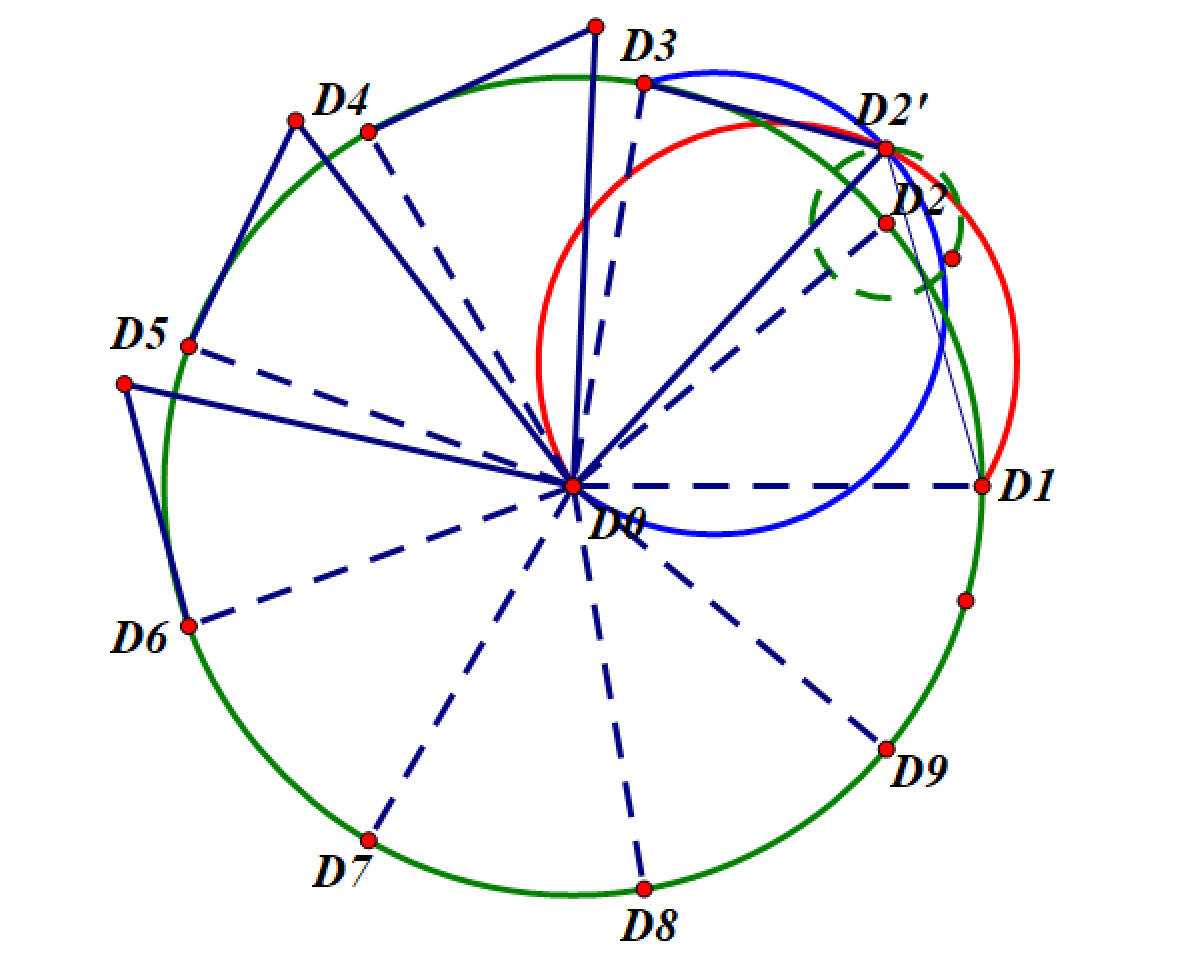
\includegraphics[width=0.5\linewidth]{./figures/3}
				\caption{$\angle D_3D_2D_0$ 的可行域$\overset{\frown}{D_3D_2D_0}$与$\angle D_0D_2D_1$ 的可行域$\overset{\frown}{D_0D_2D_1}$}
				\label{fig3}
			\end{figure}
		
		
			如图\ref{fig3}所示,对于有微小偏差的无人机$D_2'$,当假设匿名第三者为无人机3时,有可能位置$P$。同理,分别建立匿名第三者$j=4,5,6$时,$D_2'$的可能位置,分别标记为$Q,R,S$,如图\ref{fig4}.
			
			\begin{figure}[htb]
				\centering
				\subfloat[所有可能可行域集合]{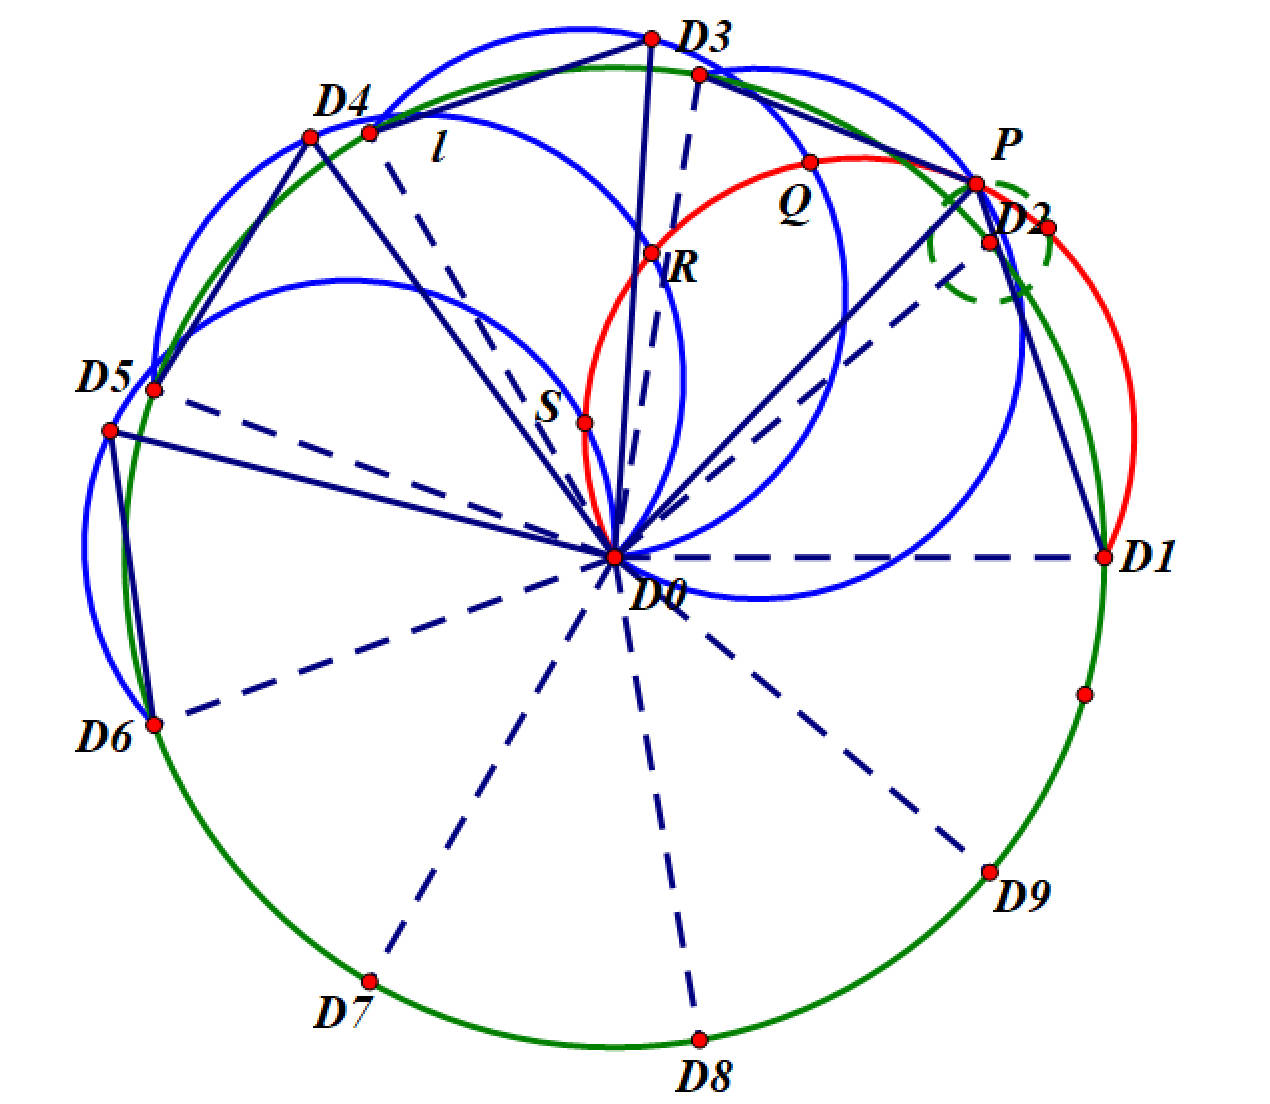
\includegraphics[width=0.4\linewidth]{../figures/4}}
				\subfloat[$D_2'$的可能位置$P,Q,R$]{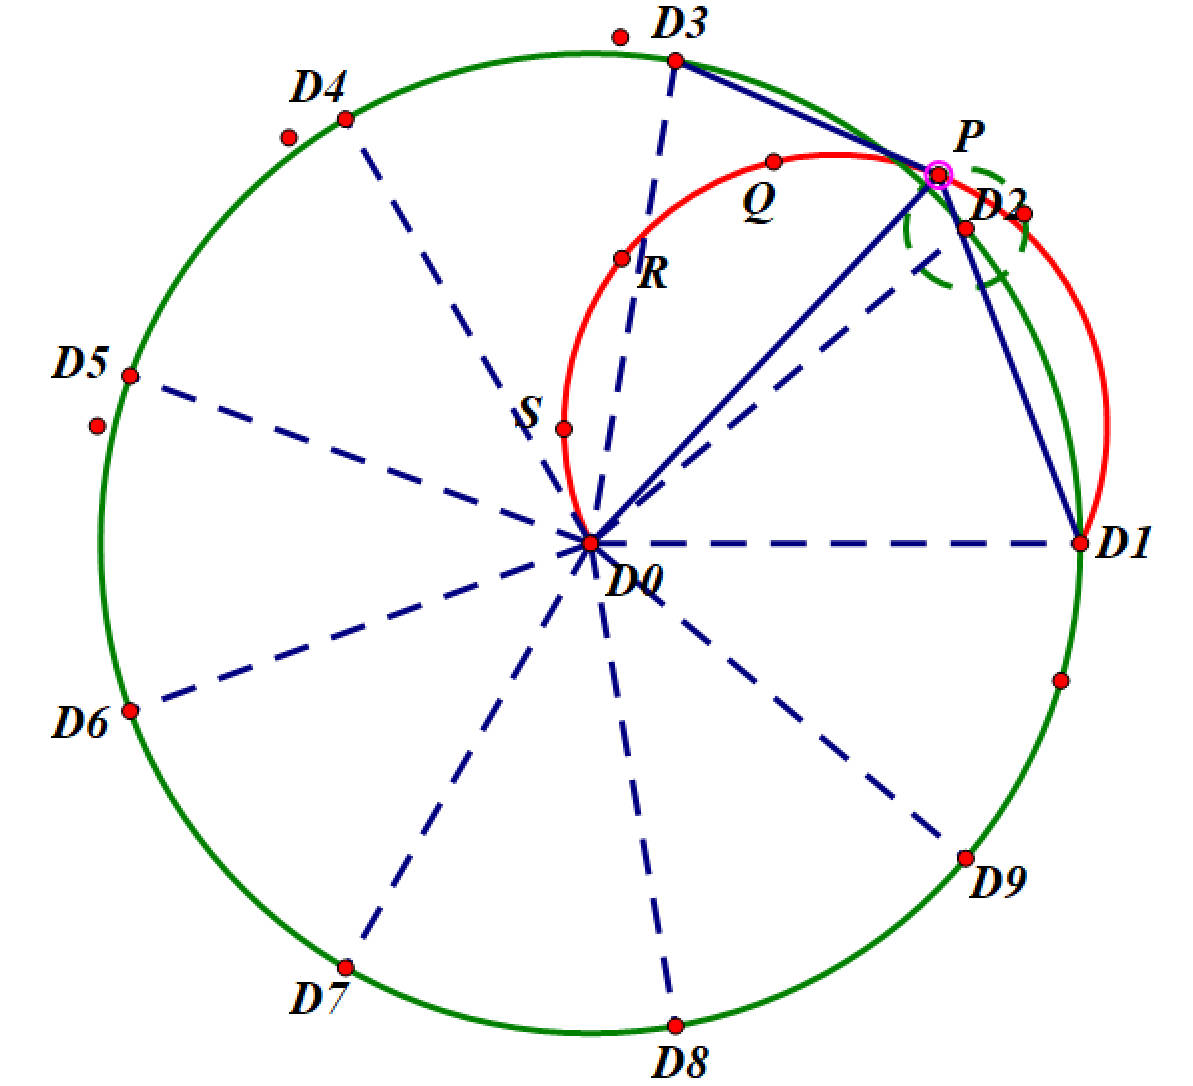
\includegraphics[width=0.4\linewidth]{../figures/5}}
				\caption{$D_2'$的可能位置的求解}
				\label{fig4}
			\end{figure}
			
			至此,对于不确定匿名第三者的情形,飞机$D_i$($D_2$)由于不能确定第三者编号产生了自己的位置猜测$P,Q,R,S$,在图\ref{fig4}的情形下,易确定$R,S$的情形不符合题设从而排除,然而我们观察到当2号机偏差很大时(即$\lVert\omega_i\rVert =\overrightarrow{D_2D_2'} $很大时)有可能出现情形如图\ref{fig6}.此时若认为第三者为4号机,则会有位置错误估计Q,然而在此种情形下,我们认为其实际位置应为图中P点的位置。因为此种情况的出现,我们要对“偏差较小”进行数学定义。
			\begin{figure}[htb]
				\centering
				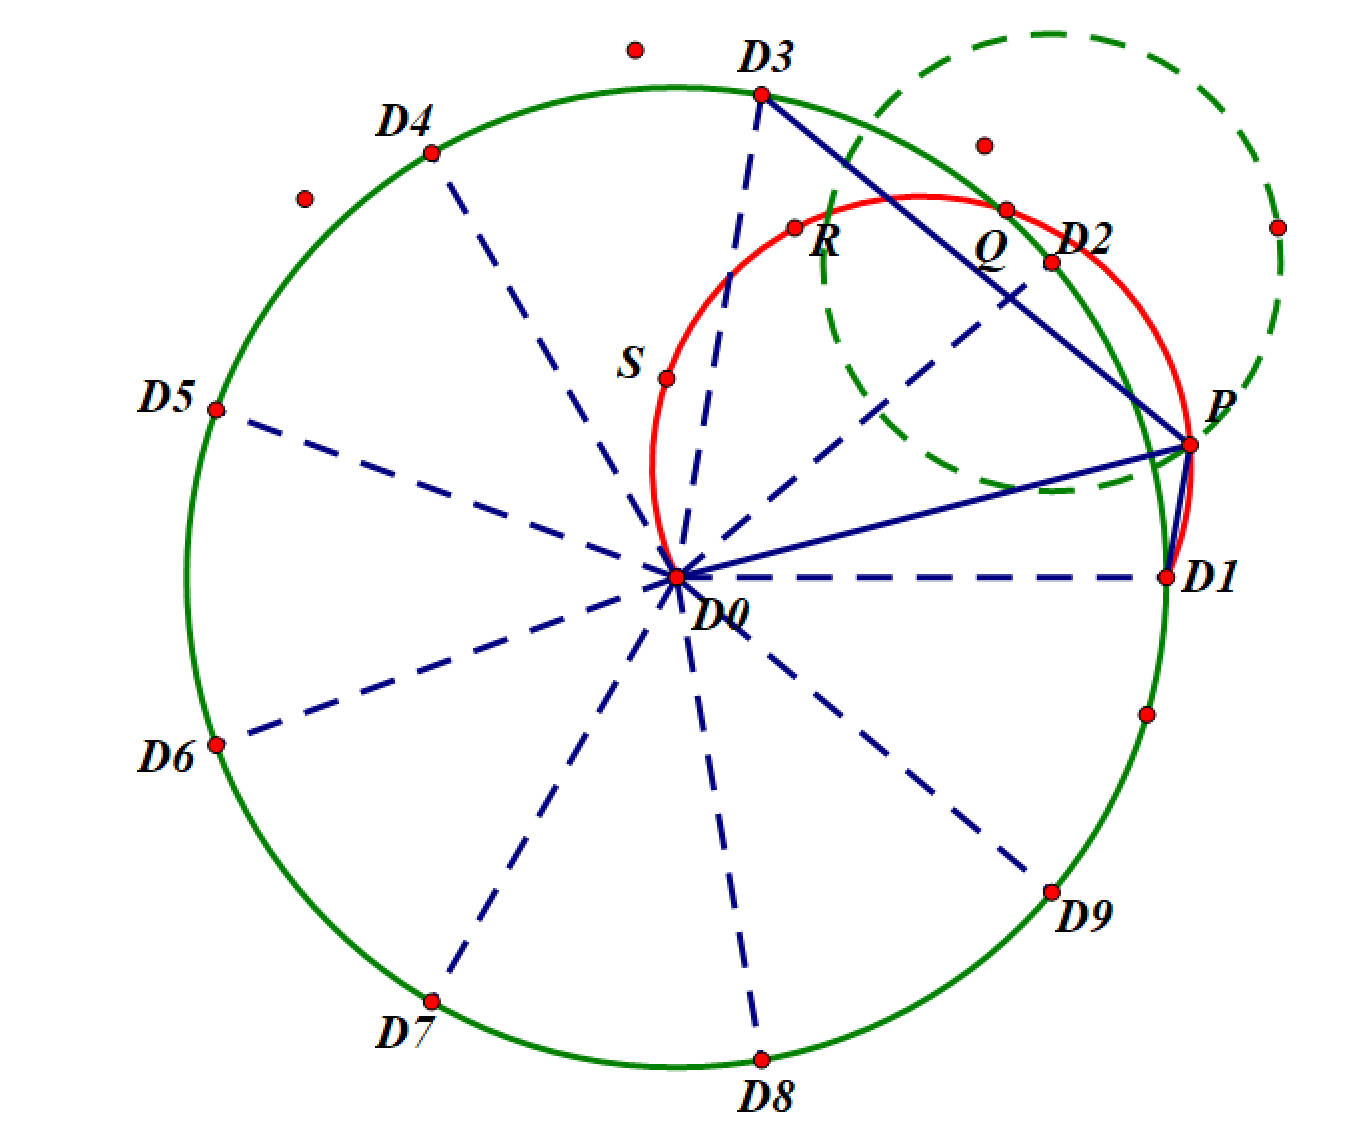
\includegraphics[width=0.5\linewidth]{./figures/6}
				\caption{偏差很大时的一种特殊情况}
				\label{fig6}
			\end{figure}
		
		
			\paragraph{多解分析}
			因为在三架飞机定位的模式下,匿名第三者未知。这种情况下待定位飞机对于自己的位置估计就可能出现多解的情况。然而我们发现,在待定位飞机距离无偏差位置很远的时候,不能通过解的合理性排除多解情况。所以我们进一步探索了多解的可排除情况的边界条件。
			
			
			当$ D_2' $ 运动在区域:$ \lVert \omega _2 \rVert \le r_0 $ 内时,$ \text{运动点}P\text{、}Q\text{、}R\text{、}S\text{的集合分别记为}\mathcal{P}\text{、}\mathcal{Q}\text{、}\mathcal{R}\text{、}\mathcal{S} $ 建立动态几何解析模型,使$ D_2' $在其运动区域边界上运动时,跟踪$P,Q,R,S$的轨迹,其内部即为$\mathcal{P}\text{、}\mathcal{Q}\text{、}\mathcal{R}\text{、}\mathcal{S}$.
			
			\begin{figure}[htb]
				\centering
				\subfloat[$r_0$很小时的运动轨迹情况]{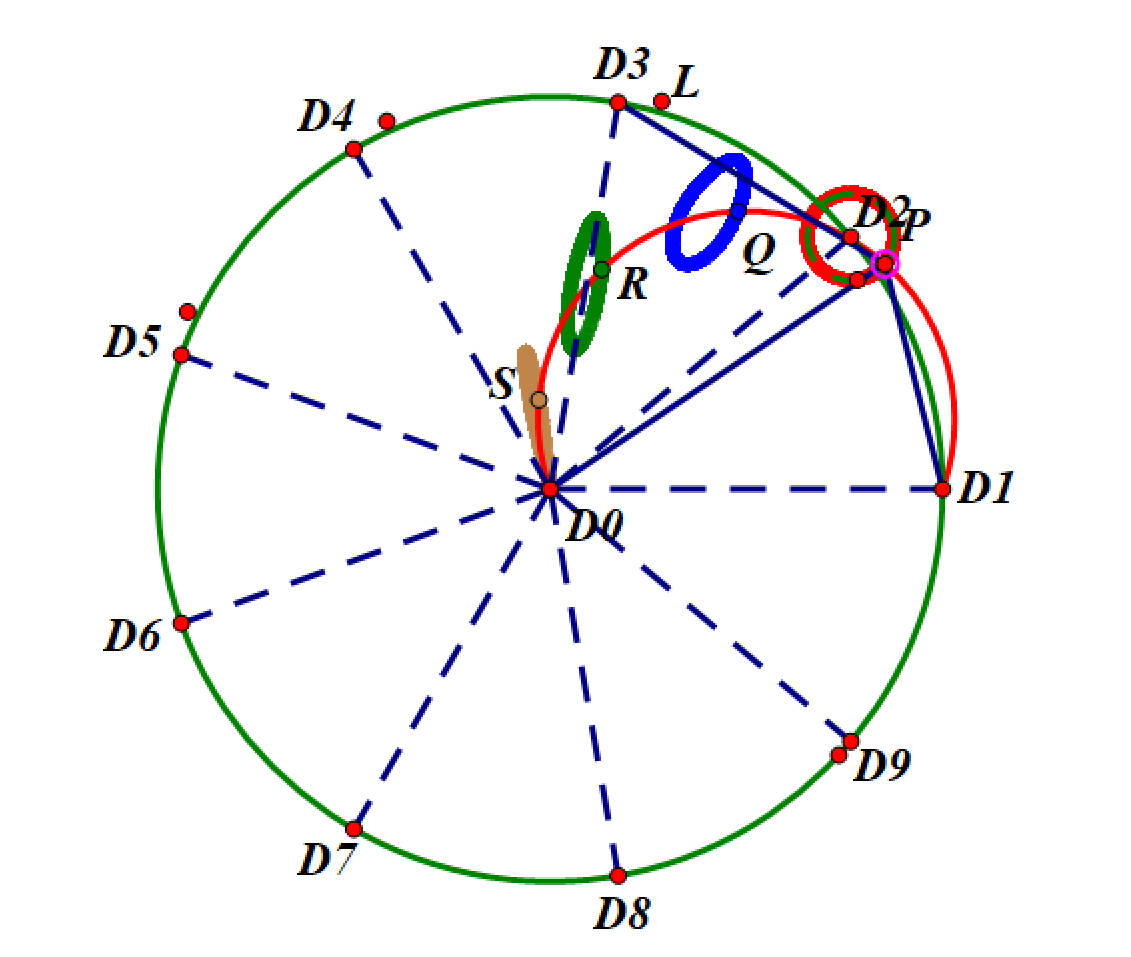
\includegraphics[width=0.43\linewidth]{../figures/7}}
				\subfloat[$r_0$处于临界时的运动轨迹情况]{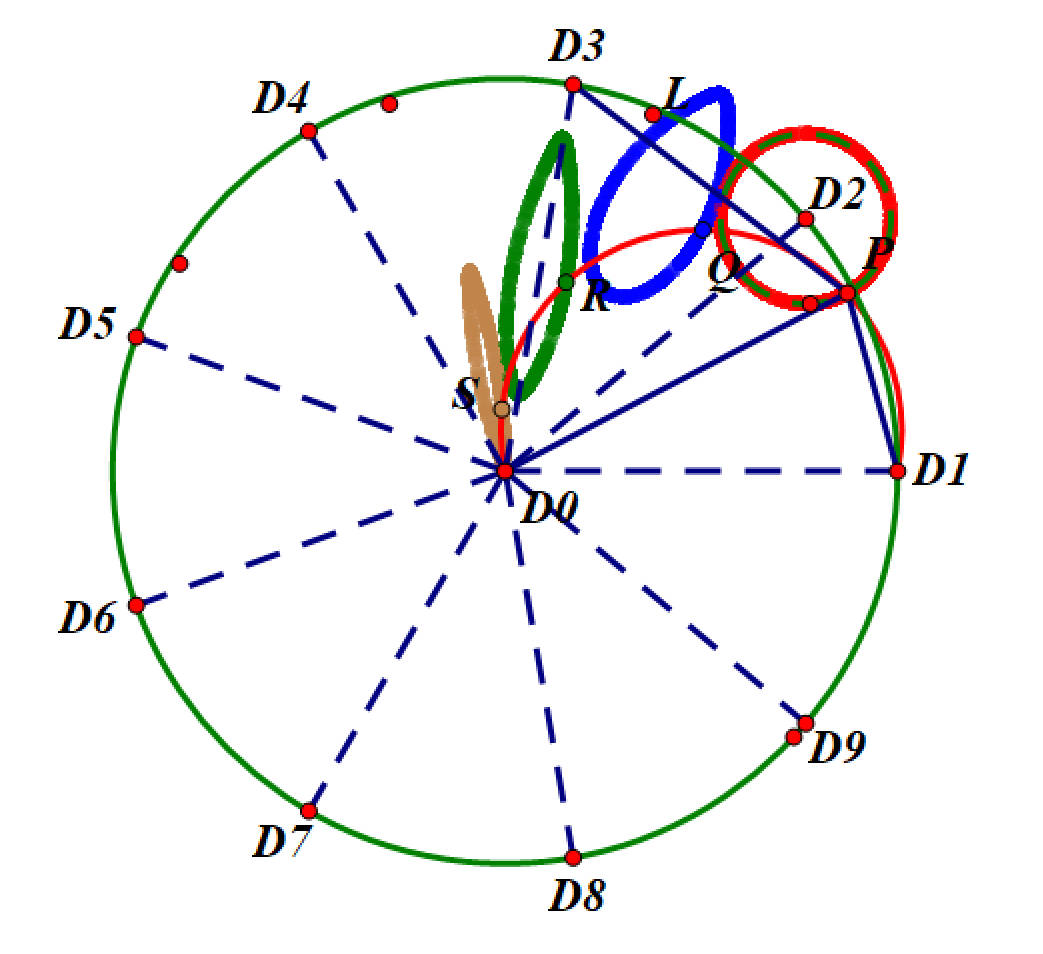
\includegraphics[width=0.4\linewidth]{../figures/8}}
				\\
				\subfloat[$r_0$很大时的运动轨迹情况]{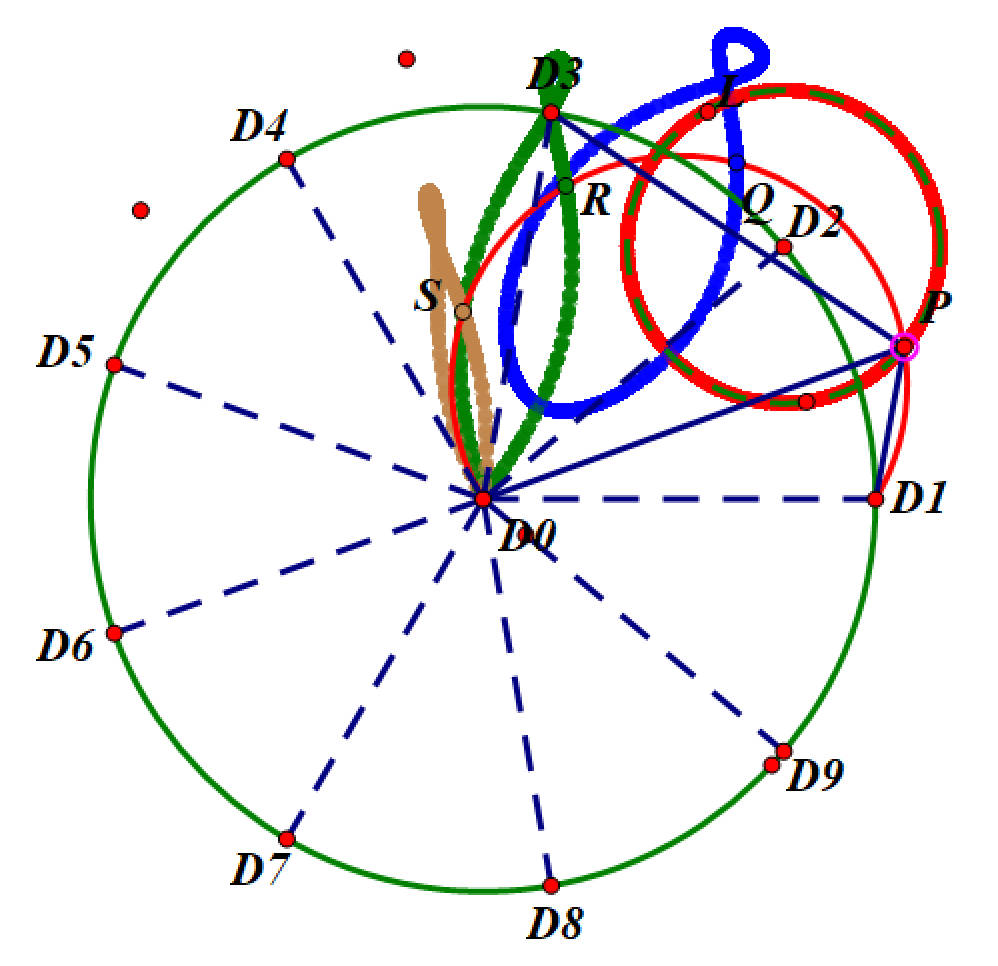
\includegraphics[width=0.4\linewidth]{../figures/9}}
				\caption{}
				\label{fig7}
			\end{figure}
			可以看出,$r_0$很大时,
			\subsubsection{title}
			\subsubsection{title}
		\subsection{问题三}
			\subsubsection{title}
			\subsubsection{title}
			\subsubsection{title}
	\section{总结}
	\begin{thebibliography}{9}%宽度9
		\bibitem{bib:one} ....
	\end{thebibliography}
	\begin{appendices}
		附录的内容。
	\end{appendices}
\end{document}